\newpage
\section{Terrain}
\begin{figure}[!ht]
  \centering
  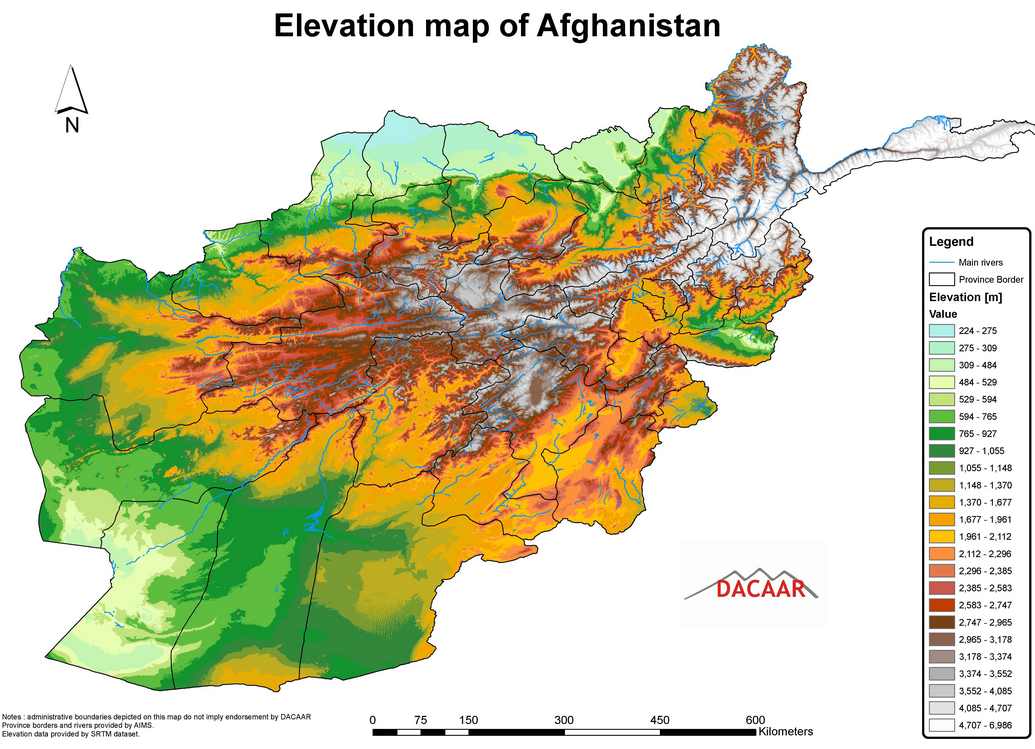
\includegraphics[width=\textwidth]{00 - Images/afghan-topography.png}
  \caption{Elevation Map Of Afghanistan \cite{afghan-topo}}
  \label{fig:af_elev}
\end{figure}

When discussing robot locomotion, it is important to analyse the threats that the physical geography might pose to the logistic tasks that the robot has to do, with a slight focus on the country with the highest amount of casualties due to landmines, more specifically Afghanistan figure \ref{fig:af_elev} shows  %that there is a shifting terrain but mainly it is mountainous and rugged. 


